\chapter{System Description}\label{chap:systemDescribtion}
The overall idea for the system is that, now one satellite is flying around Earth, but what if more satellites will be added in order to fly in formation, with a certain distance in between and with the purpose of maintaining that distance by exchanging information. As a proof of concept, an AAU-CubeSat will be used, by choosing six AAU-CubeSat that orbit the Earth like is shown in  \figref{fig:1}. Therefore, a control system is developed, where the six satellites are nodes and they represent periods, where you cannot communicate with them, so there is no active control between them. In this project, all CubeSat's will be assumed identical, where each satellite needs to fulfill a few requirements stated in \chapref{chap:requirements}. Moreover, a full-scale implementation of the system will not be possible, therefore, the whole system will be simulated using MATLAB and Simulink. 
%
\begin{figure}[H]
	\centering
	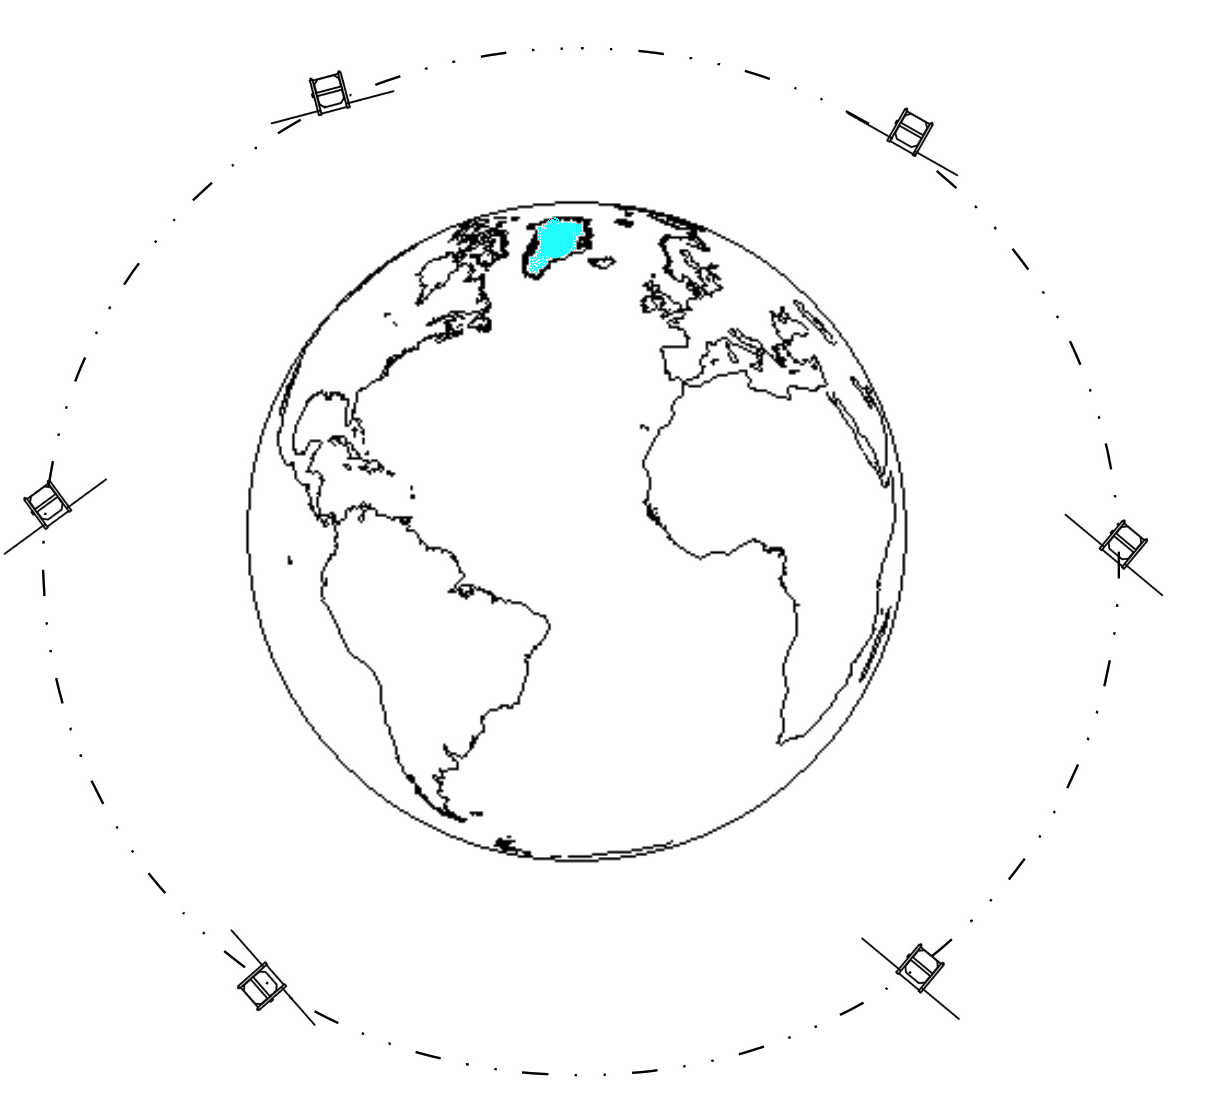
\includegraphics[width=0.6\linewidth]{figures/earth}
	\caption{desc.}
	\label{fig:1}
\end{figure}
%
The project will focus on orbital dynamics model, by looking at two satellites that are flying close to each other and study the relative dynamics.
%
\section{About AAU-CubeSat}
The AAU-CubeSat shown in \figref{fig:pico} is a pico-satellite developed by Stanford University, but assembled at Aalborg University by students and used mainly for Low Earth Orbit (LEO)  tests.
\begin{figure}[H]
	\centering
	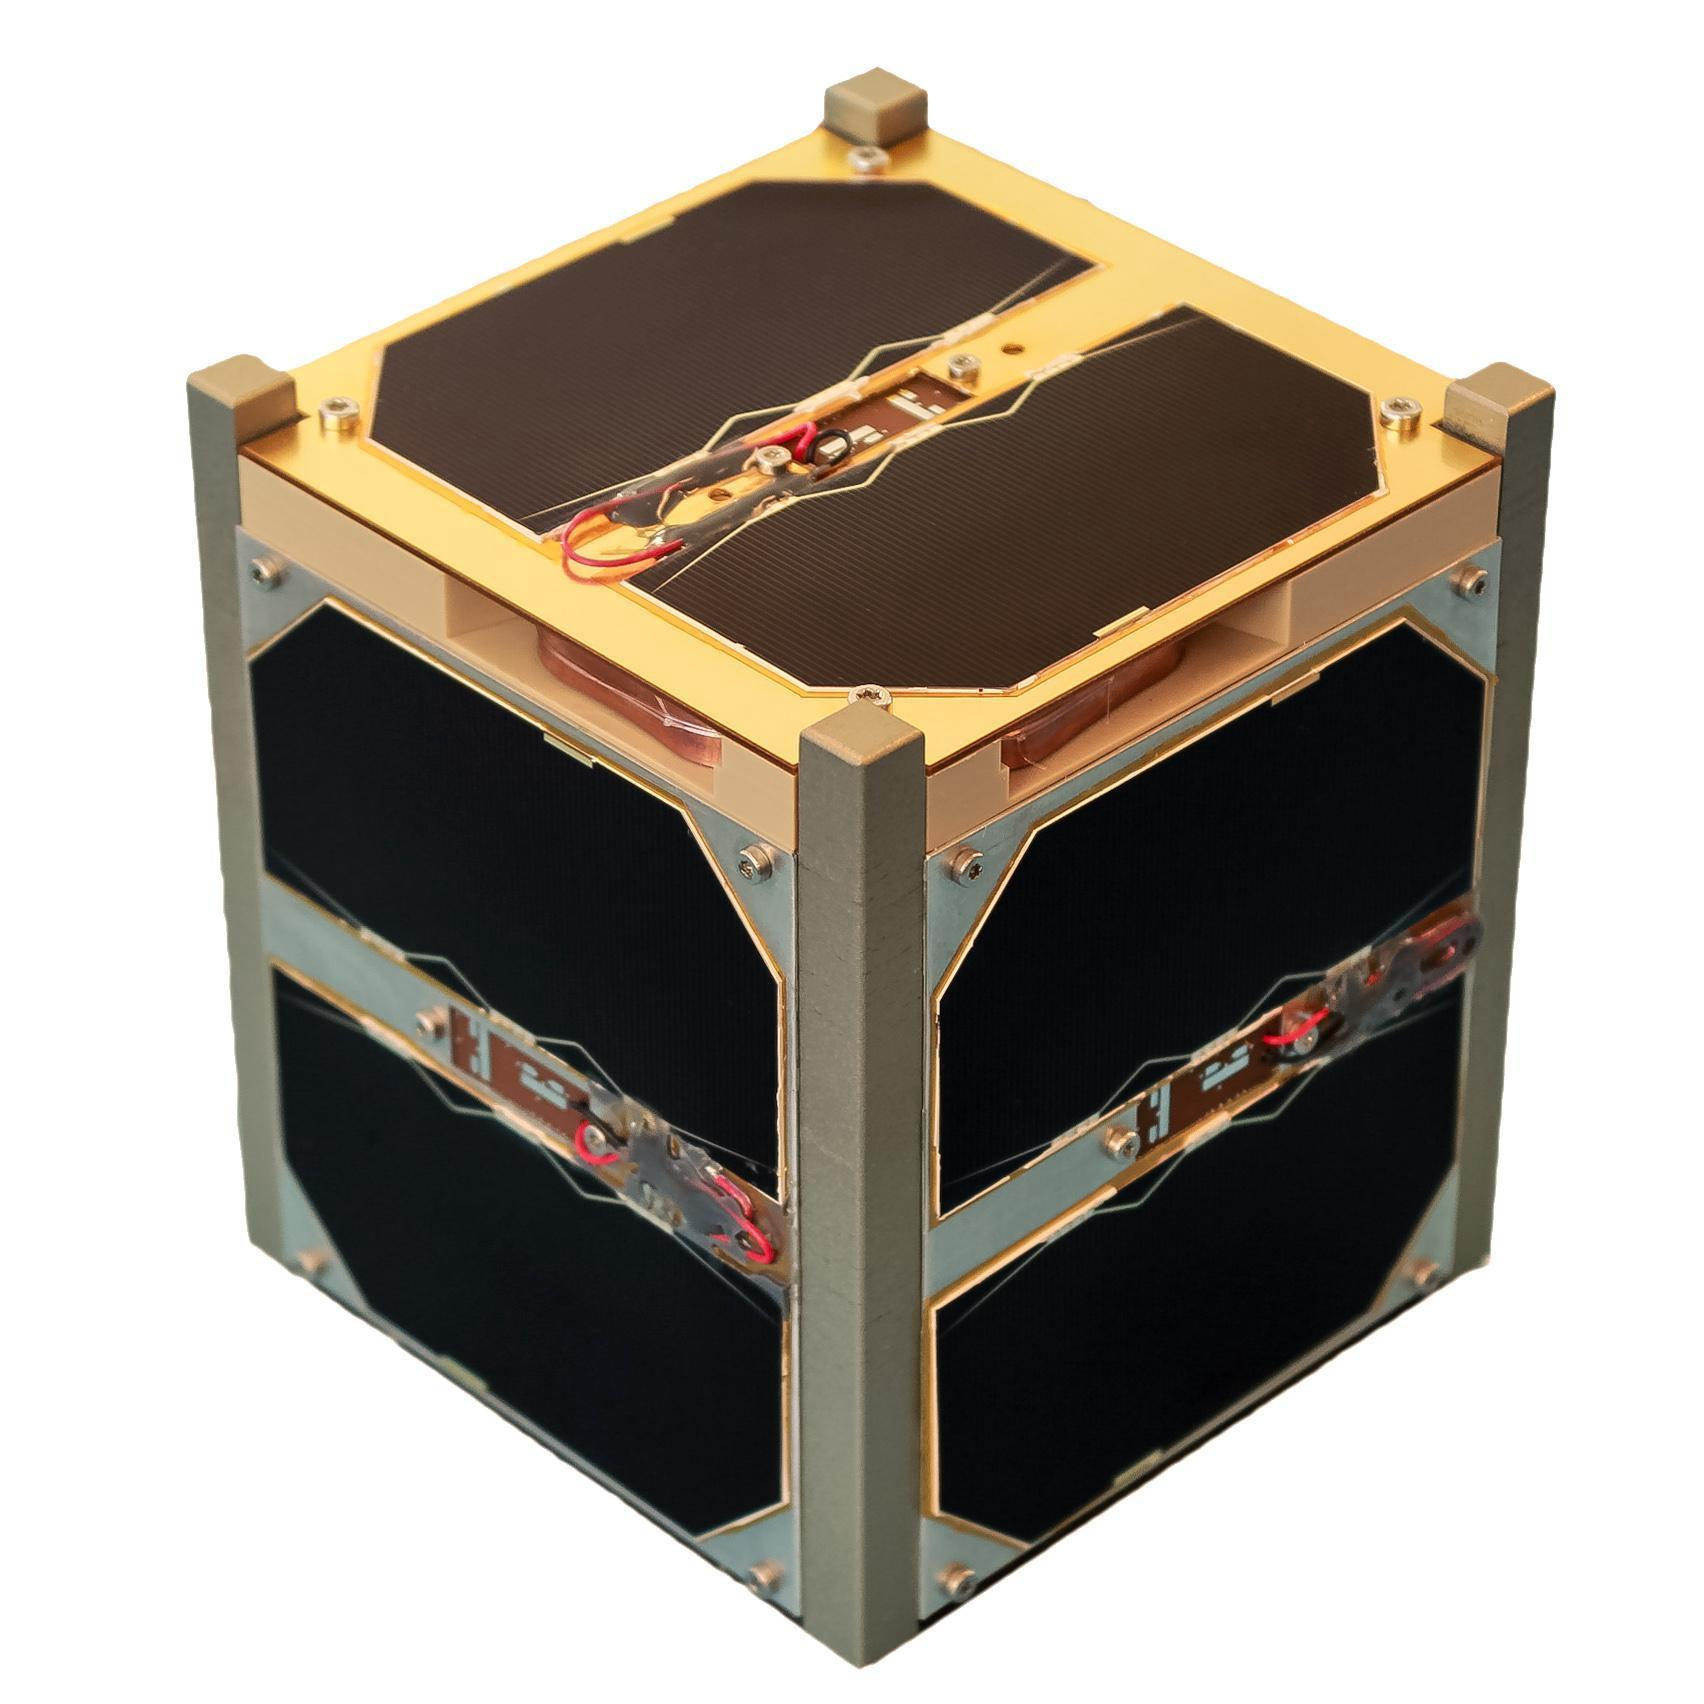
\includegraphics[width=0.3\linewidth]{figures/aau_cubsat}
	\caption{descrip}
	\label{fig:pico}
\end{figure}
The pico-satellite is designed for LEO, therefore a few constraints are imposed. The CubeSat is limited in size and weight. The dimensions of the satellite must be $10cm\times10cm\times10cm$, while the weight around 1 kg. \fxnote{ref}

In order place the CubeSat on the orbit, a deployment system is used, called P-POD \fxnote{ref} This system uses the force of a spring to launch the satellite into space. The satellite will be placed inside the launch rocket as payload. By using this system, an important advantage is reducing the cost of the launch.
%
\section{AAU-CubeSat actuators}
The selection of attitude control components is important in order to meet the performance requirements. For this project, three magnetorquers and three momentum wheels have been chosen as actuators. Initially, using only three magnetorquers has been considered, but the downside of using only momentum wheels is that some amount of torque can be stored in the wheel, which will imply to have a way to take back all that momentum and use it. Therefore, there are two ways to release that torque, one is to use magnetorquers and the second to use thrusters. \fxnote{ref}

\textbf{Magnetorquers} are wire coils which generate an electromagnetic field. The field interacts with the Earth magnetic field and a torque is generated for stabilizing the satellite. An important aspect of the magnetorquer is when the momentum wheel reaches a maximum speed and can no longer produce the torque (this is referred as wheel saturation'), so a magnetorquer is used to extract the momentum from the wheel.
%
\begin{table}[H]
	\begin{minipage}[b]{0.49\linewidth}
		\centering
		\begin{figure}[H]
			\centering
			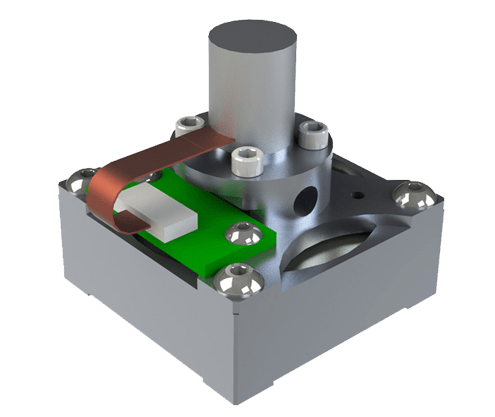
\includegraphics[width=0.5\linewidth]{figures/MW}
			\caption{Example of a reaction wheel for CubeSats}
			\label{fig:MW}
		\end{figure}
	\end{minipage}\hfill
	\begin{minipage}[b]{0.49\linewidth}
		\centering
		\begin{figure}[H]
			\centering
			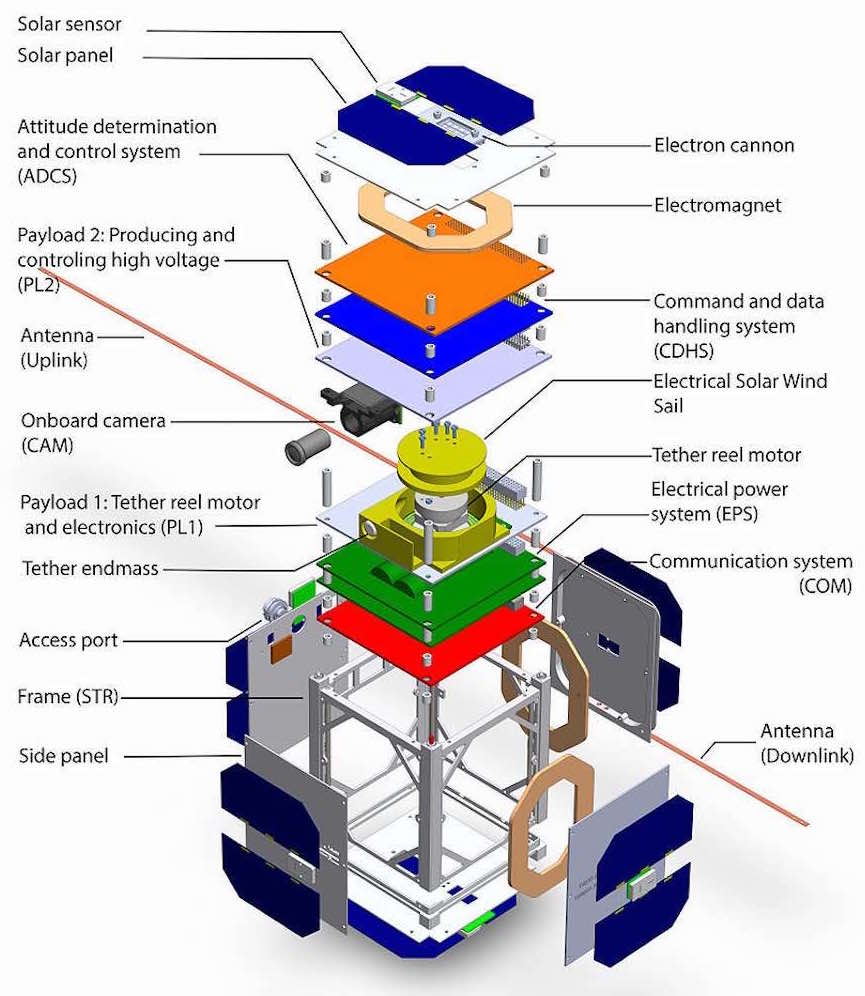
\includegraphics[width=1\linewidth]{figures/cubsat}
			\caption{Cubesat 3D view}
			\label{fig:cub}
		\end{figure}
	\end{minipage}
\end{table}
%
\textbf{Momentum wheels} shown in \figref{fig:MW} strength is that no information is needed about the magnetic field in order to control the CubeSat torque. These wheels are capable to store the momentum needed for maneuvering or pointing.
%
\section{AAU-CubeSat sensors}
On the CubeSat is sitting solar pannels [ref in fig 2.4] with in the middle a sun sensor, which provide a vector equal to the direction of the sun and also a magnetometer that gives a vector of the Earth's magnetic field. Whether the Earth’s magnetic field is measured, or the sun vector, the objective is to use these sensors to deliver vector solutions for determining the satellite’s pointing and rota- tion rates.

\textbf{Magnetometer} is a sensor used for attitude control, which measure the direction and intensity of the magnetic field. The atittude is determined from the magnetometer by comparing the measure magnetic field with a referance field.

\textbf{Sun sensor} is used for delivering a vector of measurements from the Sun. (ref to the fig 2.4 )

\textbf{GPS} provide the position of the satellite. (maybe not needed since we use a orbit model to find the position of the satellite !!)

\textbf{Earth Horizon Sensor } \\
\textbf{Star tracker}\\
\textbf{Camera}
%
\section{Pointing accuracy}
The required pointing accuracy when acquiring a photo is based on the a height from the picture is taken, in this case around 700 km above the Earth surface is going to cover approximately ?? km. 



